% Unofficial UChicago CS Poster Template
% v1.1.0 released September 8, 2022
% https://github.com/k4rtik/uchicago-poster
% a fork of https://github.com/anishathalye/gemini

\documentclass{beamer}

% ====================
% Packages
% ====================

\usepackage[T1]{fontenc}
\usepackage{lmodern}
\usepackage[size=custom,width=80,height=120,scale=1.0]{beamerposter}
\usetheme{gemini}
\usepackage{graphicx}
\usepackage{booktabs}
\usepackage{doi}
\usepackage[numbers]{natbib}
\usepackage[patch=none]{microtype}
\usepackage{tikz}
\usepackage{pgfplots}
\pgfplotsset{compat=1.18}
\usepackage{anyfontsize}
\usepackage{subcaption}

\definecolor{violet}{RGB}{80, 60, 100}

\setbeamercolor{headline}{fg=white,bg=violet}
\setbeamercolor{palette primary}{fg=black,bg=white}
\setbeamercolor{palette secondary}{fg=black,bg=white}
\setbeamercolor{palette tertiary}{bg=black,fg=white}
\setbeamercolor{palette quaternary}{fg=black,bg=white}
\setbeamercolor{structure}{fg=black}

% ====================
% Lengths
% ====================

% If you have N columns, choose \sepwidth and \colwidth such that
% (N+1)*\sepwidth + N*\colwidth = \paperwidth
\newlength{\sepwidth}
\newlength{\colwidth}
\setlength{\sepwidth}{0.025\paperwidth}
\setlength{\colwidth}{0.45\paperwidth}

\newcommand{\separatorcolumn}{\begin{column}{\sepwidth}\end{column}}

% ====================
% Title
% ====================

\title{Power law attention biases for molecular transformers}

\author{Jay Shen \inst{1}\inst{2} \and Oliver Tang \inst{1}\inst{3} \and Andrew Ferguson \inst{1}\inst{3}}

\institute[shortinst]{\inst{1} University of Chicago \inst{2} Department of Physics \inst{3} School of Molecular Engineering}

% ====================
% Footer (optional)
% ====================

\footercontent{
  \href{https://github.com/jshe2304/molecular_attention_bias}{https://github.com/jshe2304/molecular\_attention\_bias}
  \hfill
  NeurIPS Machine Learning for Physical Sciences Workshop 2025
  \hfill
  \href{mailto:jshe@uchicago.edu}{jshe@uchicago.edu}
}

% ====================
% Logo (optional)
% ====================

\logoright{
\includegraphics[height=7cm]{figures/qr-code.png}\hspace{5em}
\includegraphics[height=7cm]{figures/uchicago.png}\hspace{5em}
\includegraphics[height=7cm]{figures/neurips.png}\hspace{5em}}

% ====================
% Body
% ====================

\begin{document}
\begin{frame}[t]

% ----- Section 1
\vspace{-2em}
\begin{block}{}
\begin{columns}[t]

\separatorcolumn

\begin{column}{\colwidth}

    \begin{block}{Introduction}
        Transformers \cite{transformer} are the go-to architecture for most data modalities due to their scalability. While they have been applied extensively to molecular property prediction, they do not dominate the field as they do elsewhere. One cause may be the lack of structural biases that effectively capture the relationships between atoms. 
    \end{block}

    \begin{block}{Structural biases for molecular transformers}
        \begin{itemize}
            \item {
                Positional encodings are popular structural biases for transformers, but are disadvantaged in that they are associated with individual tokens rather than inter-token structure. 
            }
            \item {
                Graph attention is another popular structural bias, but is similarly disadvantaged because it cannot model 3D point cloud geometry. 
            }
            \item{
                Attention biases are added to attention logits and naturally model pairwise relationships. They can be easily constructed given some notion of inter-token distance as in \cite{gaussian-kernel}. 
                \begin{equation}\label{biased-attention}
                    A_{ij} = \text{softmax}_j \Biggr[ \frac{\mathbf{q}_{i} \mathbf{k}_j^T}{\sqrt{d_k}} + b_{ij} \Biggr]
                \end{equation}
            }
        \end{itemize}
    \end{block}

\end{column}

\separatorcolumn

\begin{column}{\colwidth}

    \begin{block}{Power law attention biases}
        We propose the following attention bias:
        \begin{equation}\label{power-law-bias}
            b_{ij} = p \log || \mathbf{r}_i - \mathbf{r}_j ||
        \end{equation}
        Because of the softmax operation, this bias term weights attention probabilities according to a power law of the interatomic distance: 
        \begin{equation}
        \begin{split}
            A_{ij} &= \text{softmax}_j \biggr [\frac{\mathbf{q}_{i} \mathbf{k}_j^T}{\sqrt{d_k}} + p \log || \mathbf{r}_i - \mathbf{r}_j || \biggr] \\
            &\propto \exp \biggr[ \frac{\mathbf{q}_{i} \mathbf{k}_j^T}{\sqrt{d_k}} + p \log || \mathbf{r}_i - \mathbf{r}_j || \biggr] \\
            &= || \mathbf{r}_i - \mathbf{r}_j ||^{p}\exp \biggr[ \frac{\mathbf{q}_{i} \mathbf{k}_j^T}{\sqrt{d_k}} \biggr]
        \end{split}
        \end{equation}
        The parameter $p$ represents the power law exponent and can be held fixed, learned per layer, or learned per attention head for varying degrees of expressivity. 
        
        The effect of this attention bias is to weight attention probabilities separately from the query-key compatibility, and to do so as a function of the interatomic distance. This is conceptually similar to physical interactions like Coulomb's law, which modulates the electric force using both particle charge and separation. 
    \end{block}

\end{column}

\separatorcolumn

\end{columns}
\end{block}

\hline
\vspace{-1em}
% ----- Section 2
\begin{block}{}
\begin{columns}[t]

\separatorcolumn

\begin{column}{\colwidth}

    \begin{block}{Experimental Setup}
        We benchmark transformers using power law attention biases on QM9 \cite{qm9} and SPICE \cite{spice}. The performance of transformers using graph attention and positional encodings are shown for comparison. Model size is kept roughly constant at 1.5M parameters across all tested models. Compute is also kept roughly constant by training all models 128 epochs. 
    \end{block}

    \begin{block}{Results}

    \begin{table}[]
        \normalsize
        \centering
        \caption{Ensemble MAE (eV) benchmarks on QM9 and SPICE}
        \begin{tabular}{l c ccccc c c}
            &&\multicolumn{5}{c}{QM9} && \multicolumn{1}{c}{SPICE} \\
            \cline{3-7}\cline{9-9}
            \noalign{\vskip 2pt}
            Structural bias && HOMO & LUMO & $U$ & $H$ & $G$ && $U_F$\\
            \hline
            \noalign{\vskip 2pt}
            Vanilla Attention \cite{transformer} && 0.34 & 0.74 & 24 (1) & 24 (1) & 24 (1) && 9 \\
            Masked Attention && 0.12 & 0.14 & 29 (4) & 29 (4) & 30 (4) && - \\
            RWPE \cite{rwpe} && 0.14 & 0.20 & 42 (7) & 42 (7) & 42 (8) && - \\
            Gaussian Kernel \cite{gaussian-kernel} && 0.08 & 0.10 & 21 (1) & 21 (1) & 21 (1) && - \\
            Power law $p=-1$ && 0.11 & 0.13 & 26 (1) & 26 (1) & 26 (1) && 7 (1) \\
            Power law $p \in \mathbb{R}$ && 0.12 & 0.14 & 25 (1) & 25 (1) & 25 (1) && 5 (1) \\
            Power law $p\in \mathbb{R}_-$ && 0.11 & 0.12 & 21 (1) & 21 (1) & 21 (1) && 5 (1) \\
        \end{tabular}
        \label{tab:mae}
    \end{table}

    In our experiments described in \ref{tab:mae}, we find that attention biases consistently outperform other structural biases. Of the attention biases, Gaussian kernel biases are the most performant in general, but power law biases where $p\in\mathbb{R}^-$ come very close at a much lower complexity. 
    
    It makes sense why this power law is superior to $p=-1$ and $p\in\mathbb{R}$, as it is more expressive than the former and more physically principled than the latter. Learned exponents follow no interpretable pattern, as shown below:

    \begin{figure}
        \centering
        \begin{subfigure}[t]{0.4\textwidth}
            \centering
            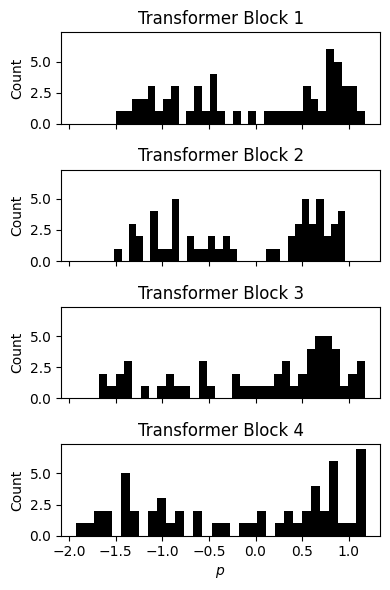
\includegraphics[width=\linewidth]{figures/exponents_unconstrained.png}
            \caption{Learned exponents $p\in\mathbb{R}$ of power law attention biases}
        \end{subfigure}%
        \hspace{2.5em}
        \begin{subfigure}[t]{0.4\textwidth}
            \centering
            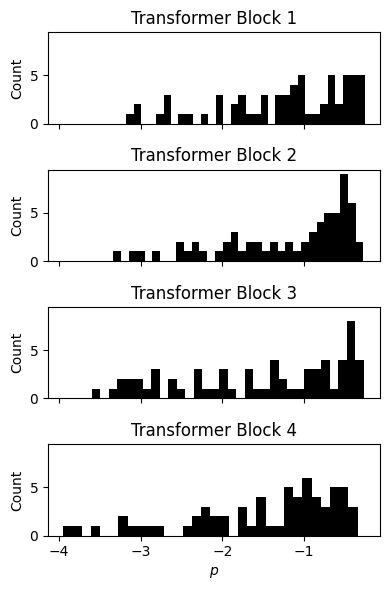
\includegraphics[width=\linewidth]{figures/exponents_negative.png}
            \caption{Learned exponents $p\in\mathbb{R}^-$ of power law attention biases}
        \end{subfigure}
    \end{figure}
    
    \end{block}

\end{column}

\separatorcolumn

\begin{column}{\colwidth}

    \begin{block}{Ablation study}

        Consider ablating the scaled dot-product so attention is only a function of the attention bias:
        \begin{equation}\label{fixed-attention}
            A_{ij} = \text{softmax}_j \big[ b_{ij} \big]
        \end{equation}
        Here, information flow is independent of token embeddings, and the attention mechanism reduces to message-passing on a complete graph. 
        \begin{table}[]
            \normalsize
            \centering
            \caption{Ensemble MAE loss of ablated models with standard deviations in parentheses. }
            \begin{tabular}{l c ccccc}
                Attention Bias && HOMO & LUMO & $U$ & $H$ & $G$ \\
                \hline
                \noalign{\vskip 2pt}
                Gaussian kernel &&  0.09 & 0.11 & 20 (2) & 20 (2) & 20 (2) \\
                Power law $p=-1$ && 0.13 & 0.16 & 27 (3) & 27 (3) & 27 (3) \\
                Power law $p\in \mathbb{R}$ && 0.12 & 0.14 & 25 (2) & 25 (2) & 25 (2) \\
                Power law $p \in \mathbb{R}_-$ && 0.11 & 0.13 & 25 (3) & 25 (3) & 25 (3) \\
            \end{tabular}
            \label{tab:ablating-attention}
        \end{table}
    
        As shown in Table \ref{tab:ablating-attention}, ablating the dot-product generally increases loss by a few eV. But in the case of the Gaussian kernal bias, loss actually decreases for $U$, $H$, and $G$! 
        
        Thus, attention biases themselves contain a fair amount of modeling capacity. They can act as cheap, reasonably good substitutes for attention itself. 

        \begin{figure}
            \centering
            \begin{subfigure}[t]{0.4\textwidth}
                \centering
                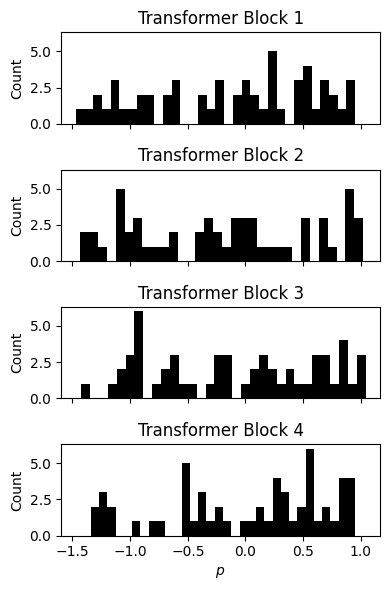
\includegraphics[width=\linewidth]{figures/exponents_unconstrained_fixed.png}
                \caption{Learned exponents $p\in\mathbb{R}$ of power law attention bias with ablated dot-products}
            \end{subfigure}%
            \hspace{2.5em}
            \begin{subfigure}[t]{0.4\textwidth}
                \centering
                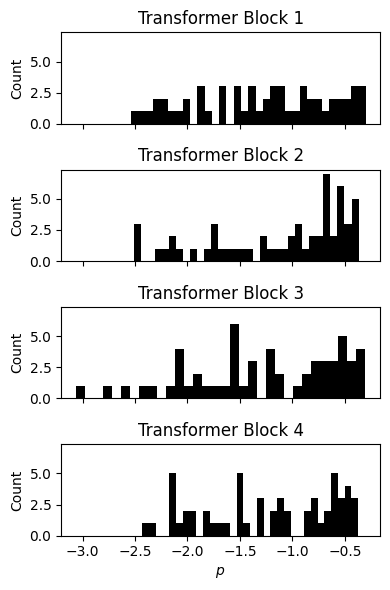
\includegraphics[width=\linewidth]{figures/exponents_negative_fixed.png}
                \caption{Learned exponents $p\in\mathbb{R}^-$ of power law attention bias with ablated dot-products}
            \end{subfigure}
        \end{figure}
    
    \end{block}

    \begin{block}{References}
    
        \begin{thebibliography}{9}
            \footnotesize
    
            \bibitem{transformer}
            A.~Vaswani.
            \textit{Attention is all you need}.
            2017.
    
            \bibitem{qm9}
            R.~Ramakrishnan.
            \textit{Quantum chemistry structures and properties of 134 kilo molecules}.
            2014.
    
            \bibitem{spice}
            P.~Eastman.
            \textit{Spice, a dataset of drug-like molecules and peptides for training machine learning potentials}.
            2022.
    
            \bibitem{gaussian-kernel}
            S.~Luo.
            \textit{One transformer can understand both 2d and 3d molecular data}.
            2023.
            
            \bibitem{rwpe}
            V.~P. Dwivedi.
            \textit{Graph neural networks with learnable structural and positional representations}.
            2022.
    
        \end{thebibliography}

    \end{block}

\end{column}

\separatorcolumn

\end{columns}
\end{block}

\end{frame}

\end{document}